%% NSS-MIC_Instructions.tex
%% 8/2007
%% By Bo Yu (yu@bnl.gov)
%% based on:
%% bare_jrnl.tex
%% V1.3
%% 2007/01/11
%% by Michael Shell
%% see http://www.michaelshell.org/
%% for current contact information.
%%
%% This is a skeleton file demonstrating the use of IEEEtran.cls
%% (requires IEEEtran.cls version 1.7 or later) with an IEEE journal paper.
%%
%% Support sites:
%% http://www.michaelshell.org/tex/ieeetran/
%% http://www.ctan.org/tex-archive/macros/latex/contrib/IEEEtran/
%% and
%% http://www.ieee.org/


%%*************************************************************************
%% Legal Notice:
%% This code is offered as-is without any warranty either expressed or
%% implied; without even the implied warranty of MERCHANTABILITY or
%% FITNESS FOR A PARTICULAR PURPOSE! 
%% User assumes all risk.
%% In no event shall IEEE or any contributor to this code be liable for
%% any damages or losses, including, but not limited to, incidental,
%% consequential, or any other damages, resulting from the use or misuse
%% of any information contained here.
%%
%% All comments are the opinions of their respective authors and are not
%% necessarily endorsed by the IEEE.
%%
%% This work is distributed under the LaTeX Project Public License (LPPL)
%% ( http://www.latex-project.org/ ) version 1.3, and may be freely used,
%% distributed and modified. A copy of the LPPL, version 1.3, is included
%% in the base LaTeX documentation of all distributions of LaTeX released
%% 2003/12/01 or later.
%% Retain all contribution notices and credits.
%% ** Modified files should be clearly indicated as such, including  **
%% ** renaming them and changing author support contact information. **
%%
%% File list of work: IEEEtran.cls, IEEEtran_HOWTO.pdf, bare_adv.tex,
%%                    bare_conf.tex, bare_jrnl.tex, bare_jrnl_compsoc.tex
%%*************************************************************************
\documentclass[journal]{IEEEtran}
\usepackage{graphicx}

\begin{document}
\title{Dirac integration with a general purpose bookkeeping DB: a complete general suite for distributed resources exploitation}
%
% author names and IEEE memberships
% note positions of commas and nonbreaking spaces ( ~ ) LaTeX will not break
% a structure at a ~ so this keeps an author's name from being broken across
% two lines.
% use \thanks{} to gain access to the first footnote area
% a separate \thanks must be used for each paragraph as LaTeX2e's \thanks
% was not built to handle multiple paragraphs
%

\author{F~Bianchi,~\IEEEmembership{INFN,}
        M~Chrzaszcz,~\IEEEmembership{IFJ PAN,}
        V~Ciaschini,~\IEEEmembership{INFN,}
        M~Corvo,~\IEEEmembership{INFN,}
        C~De~Santis,~\IEEEmembership{INFN,}
        D~Del~Prete,~\IEEEmembership{INFN,}
        A~Di~Simone,~\IEEEmembership{INFN,}
        G~Donvito,~\IEEEmembership{INFN,}
        A~Fella,~\IEEEmembership{INFN,}
        P~Franchini,~\IEEEmembership{INFN,}
        F~Giacomini,~\IEEEmembership{INFN,}
        A~Gianelle,~\IEEEmembership{INFN,}
        R~Grzymkowski,~\IEEEmembership{IFJ PAN,}        
        S~Longo,~\IEEEmembership{INFN,}        
        S~Luitz,~\IEEEmembership{SLAC,}        
        E~Luppi,~\IEEEmembership{INFN,}               
        M~Manzali,~\IEEEmembership{INFN,}
        M~Rama,~\IEEEmembership{INFN,}
        G~Russo,~\IEEEmembership{INFN,}
        S~Pardi,~\IEEEmembership{INFN,}
        L~Perez,~\IEEEmembership{INFN,}
        B~Santeramo,~\IEEEmembership{INFN,}
        R~Stroili,~\IEEEmembership{INFN,}
        L~Tomassetti,~\IEEEmembership{INFN,}        
        and~M~Zdybal,~\IEEEmembership{IFJ PAN}% <-this % stops a space

\thanks{F. Bianchi is with University of Torino, Turin, Italy and INFN - Sezione di Torino, Turin, Italy}%
\thanks{M~Chrzaszcz is with Physik-Institut, Universitat Zurich, Zurich, Switzerland and Henryk Niewodniczanski Institute of Nuclear Physics Polish Academy of Sciences, Krakow, Poland}%
\thanks{V~Ciaschini is with INFN - CNAF, Bologna, Italy}%
\thanks{M~Corvo is with INFN - Sezione di Padova, Padua, Italy}%
\thanks{C~De~Santis is with INFN - Sezione di Roma Tor Vergata, Rome, Italy and Department of Physics, University of Rome Tor Vergata, Rome, Italy}%
\thanks{D~Del~Prete is with INFN – Sezione di Napoli, Naples, Italy}%
\thanks{A~Di~Simone is with INFN - Sezione di Roma Tor Vergata, Rome, Italy and Department of Physics, University of Rome Tor Vergata, Rome, Italy}%
\thanks{G~Donvito is with INFN - Sezione di Bari, Bari, Italy}%
\thanks{A~Fella is with INFN - Sezione di Pisa, Pisa, Italy and Department of Mathematics and Computer Science, University of Ferrara, Ferrara, Italy}%
\thanks{P~Franchini is with INFN - CNAF, Bologna, Italy}%
\thanks{F~Giacomini is with INFN - CNAF, Bologna, Italy}%
\thanks{A~Gianelle is with INFN - Sezione di Padova, Padua, Italy}%
\thanks{R~Grzymkowski is with Henryk Niewodniczanski Institute of Nuclear Physics Polish Academy of Sciences, Krakow, Poland}%
\thanks{S~Longo is with INFN - Sezione di Padova, Padua, Italy}%
\thanks{S~Luitz is with SLAC, USA}%
\thanks{E~Luppi is with Department of Physics, University of Ferrara, Ferrara, Italy and INFN - Sezione di Ferrara, Ferrara, Italy}%
\thanks{M~Manzali is with Department of Physics, University of Ferrara, Ferrara, Italy and INFN - Sezione di Ferrara, Ferrara, Italy}%
\thanks{M~Rama is with INFN - Sezione di Padova, Padua, Italy}%
\thanks{G~Russo is with INFN – Sezione di Napoli, Naples, Italy}%
\thanks{S~Pardi is with INFN – Sezione di Napoli, Naples, Italy}%
\thanks{L~Perez is with INFN - Sezione di Pisa, Pisa, Italy}%
\thanks{B~Santeramo is with INFN - Sezione di Bari, Bari, Italy and Department of Physics, University and Polytechnic of Bari, Bari, Italy}%
\thanks{R~Stroili is with INFN - Sezione di Padova, Padua, Italy}%
\thanks{L~Tomassetti is with Department of Mathematics and Computer Science, University of Ferrara, Ferrara, Italy and INFN - Sezione di Ferrara, Ferrara, Italy}%
\thanks{M~Zdybal is with Henryk Niewodniczanski Institute of Nuclear Physics Polish Academy of Sciences, Krakow, Poland}%
}

\maketitle
\pagestyle{empty}
\thispagestyle{empty}

\begin{abstract}
In the context of High Energy Physics computing field the R\&D studies aimed to the definition of the data and workload models have been carried on and completed by the Super$B$ community beyond the experiment life itself. The work resulted of great interest for a generic mid- and small size VO to fulfill Grid exploiting requirements involving CPU-intensive tasks. We present the R\&D line achievements in the design, developments and test of a distributed resource exploitation suite based on DIRAC. The main components of such a suite are the information system, the job wrapper and the new generation DIRAC framework. The DB schema and the SQL logic have been designed to be able to be adaptive with respect to the VO requirements in terms of physics application, job environment and bookkeeping parameters. A deep and flexible integration with DIRAC features has been obtained using SQLAlchemy technology allowing mapping and interaction with the information system. A new DIRAC extension has been developed to include this functionality along with a new set of DIRAC portal interfaces aimed to the job, distributed resources, and metadata management. The results of the first functionality and efficiency tests will be reported.
\end{abstract}

%\begin{IEEEkeywords}
%IEEEtran, journal, \LaTeX, paper, template.
%\end{IEEEkeywords}


\section{Introduction}
% The very first letter is a 2 line initial drop letter followed
% by the rest of the first word in caps.
% 
% form to use if the first word consists of a single letter:
% \IEEEPARstart{A}{demo} file is ....
% 
% form to use if you need the single drop letter followed by
% normal text (unknown if ever used by IEEE):
% \IEEEPARstart{A}{}demo file is ....
% 
% Some journals put the first two words in caps:
% \IEEEPARstart{T}{his demo} file is ....
% 
% Here we have the typical use of a "T" for an initial drop letter
% and "HIS" in caps to complete the first word.
\IEEEPARstart{I}{n} HEP as well in other fields, a typical issue is the necessity to manage and analyze huge amount of data or simulate large amount of events.
Today several solutions are yet available for this purpose, but lot of them are developed for particular needs of a specific customer.
During Super$B$ R\&D activities, a solution useful for Super$B$ was deployed which can be easily adopted by a generic small and mid-size VO.

\section{Suite description}

In order to develop a simple, standard and long term solution, suite components (adopted or developed) should be flexible enough to be adapted in order to fulfill needs of a generic VO.\\
Suite components include DIRAC\cite{ref:dirac}, the Information System and the Job Wrapper (see figure \ref{fig:project_bird_eye}).\\
\begin{itemize}
\item DIRAC is a well known and widely adopted framework to manage Grid resources, job submission, workflow definition, user authentication, authorization and accounting.
\item The Information System holds metadata related to simulations and information about dataset structures and data placement on Grid resources. Information System relies on a PostgreSQL\cite{ref:postgres} database. DIRAC interacts with Information System via SQLAlchemy\cite{ref:sqlalchemy}.
\item The Job Wrapper, executed in bundle with jobs, updates Information System about simulations status and data placement using a REST interface. Job Wrapper is a python script.
\end{itemize}

\begin{figure}[!t]
\centering
\includegraphics[width=3.5in]{project_bird_eye_2.eps}
% where an .eps filename suffix will be assumed under latex, 
% and a .pdf suffix will be assumed for pdflatex; or what has been declared
% via \DeclareGraphicsExtensions.
\caption{Project bird's eye view.}
\label{fig:project_bird_eye}
\end{figure}

\subsection{The Dirac extension}

%DIRAC, born as LHCb MonteCarlo production software, at present time is a complete solution to deploy distributed resources, suitable for large and small communities. DIRAC manage user authentication, authorization and accounting via X509 certificates, applies VO defined scheduling policies, is capable to manage resources made available via different grids, cluster, cloud and desktop computer (via BOINC). Data management capabilities include gLite/EGI storage elements as well DIRAC Storage Elements, LCG File Catalog (LFC) as well DIRAC File Catalog (DFC). The DIRAC webportal offers both user and administrative functionalities. Interfaces can be made using DIRAC API (in python) or a language neutral RESTful interface). DIRAC is widely adopted by large and small communities.\\
DIRAC can be extended to add specific functionalities required by the user. For example in Super$B$\cite{ref:superb_tdr} needs was an interface with a PostgreSQL BookKeeping database and a webportal able to display monitoring data from this database where required. This particular DIRAC extension was named SuperBDIRAC.
%DIRAC Service is a way to export functionalities. 
In SuperBDIRAC a new service, named SBKService, provides an SQLAlchemy layer able to connect DIRAC to a generic SQL DBMS. SBKService maps the bookkeeping database using Object Relational Mapping (see section \ref{sec:db}). 
Webportal extension is designed to create and manage simulations, monitoring related jobs and sites. New functionalities integration into webportal permits to use only one interface to manage and monitor the entire stack of simulation related tasks.


% An example of a floating figure using the graphicx package.
% Note that \label must occur AFTER (or within) \caption.
% For figures, \caption should occur after the \includegraphics.
% Note that IEEEtran v1.7 and later has special internal code that
% is designed to preserve the operation of \label within \caption
% even when the captionsoff option is in effect. However, because
% of issues like this, it may be the safest practice to put all your
% \label just after \caption rather than within \caption{}.
%
% Reminder: the "draftcls" or "draftclsnofoot", not "draft", class
% option should be used if it is desired that the figures are to be
% displayed while in draft mode.
%


% Note that IEEE typically puts floats only at the top, even when this
% results in a large percentage of a column being occupied by floats.


% An example of a double column floating figure using two subfigures.
% (The subfig.sty package must be loaded for this to work.)
% The subfigure \label commands are set within each subfloat command, the
% \label for the overall figure must come after \caption.
% \hfil must be used as a separator to get equal spacing.
% The subfigure.sty package works much the same way, except \subfigure is
% used instead of \subfloat.
%
%\begin{figure*}[!t]
%\centerline{\subfloat[Case I]\includegraphics[width=2.5in]{subfigcase1}%
%\label{fig_first_case}}
%\hfil
%\subfloat[Case II]{\includegraphics[width=2.5in]{subfigcase2}%
%\label{fig_second_case}}}
%\caption{Simulation results}
%\label{fig_sim}
%\end{figure*}
%
% Note that often IEEE papers with subfigures do not employ subfigure
% captions (using the optional argument to \subfloat), but instead will
% reference/describe all of them (a), (b), etc., within the main caption.


% An example of a floating table. Note that, for IEEE style tables, the 
% \caption command should come BEFORE the table. Table text will default to
% \footnotesize as IEEE normally uses this smaller font for tables.
% The \label must come after \caption as always.
%
%\begin{table}[!t]
%% increase table row spacing, adjust to taste
%\renewcommand{\arraystretch}{1.3}
% if using array.sty, it might be a good idea to tweak the value of
% \extrarowheight as needed to properly center the text within the cells
%\caption{An Example of a Table}
%\label{table_example}
%\centering
%% Some packages, such as MDW tools, offer better commands for making tables
%% than the plain LaTeX2e tabular which is used here.
%\begin{tabular}{|c||c|}
%\hline
%One & Two\\
%\hline
%Three & Four\\
%\hline
%\end{tabular}
%\end{table}


% Note that IEEE does not put floats in the very first column - or typically
% anywhere on the first page for that matter. Also, in-text middle ("here")
% positioning is not used. Most IEEE journals use top floats exclusively.
% Note that, LaTeX2e, unlike IEEE journals, places footnotes above bottom
% floats. This can be corrected via the \fnbelowfloat command of the
% stfloats package.



% if have a single appendix:
%\appendix[Proof of the Zonklar Equations]
% or
%\appendix  % for no appendix heading
% do not use \section anymore after \appendix, only \section*
% is possibly needed

% use appendices with more than one appendix
% then use \section to start each appendix
% you must declare a \section before using any
% \subsection or using \label (\appendices by itself
% starts a section numbered zero.)
%
%\vfill

\section{Bookkeeping DB}
\label{sec:sbk}

MonteCarlo events production needs a method to identify data files and Storage Elements that holds them. 
A BookKeeping database, named SBK (Super$B$ BookKeeping), have been developed to manage metadata associated with data files. The same database stores information about simulations, executed jobs and output data, site availability in terms of installed and supported software. SBK is used also to schedule jobs submission in order to complete simulations. Database is modeled to fulfill general requirements of a typical simulation production.\\
Entities in SBK are Session, Production and Request (see figure 2).

\begin{figure}[!h]
\centering
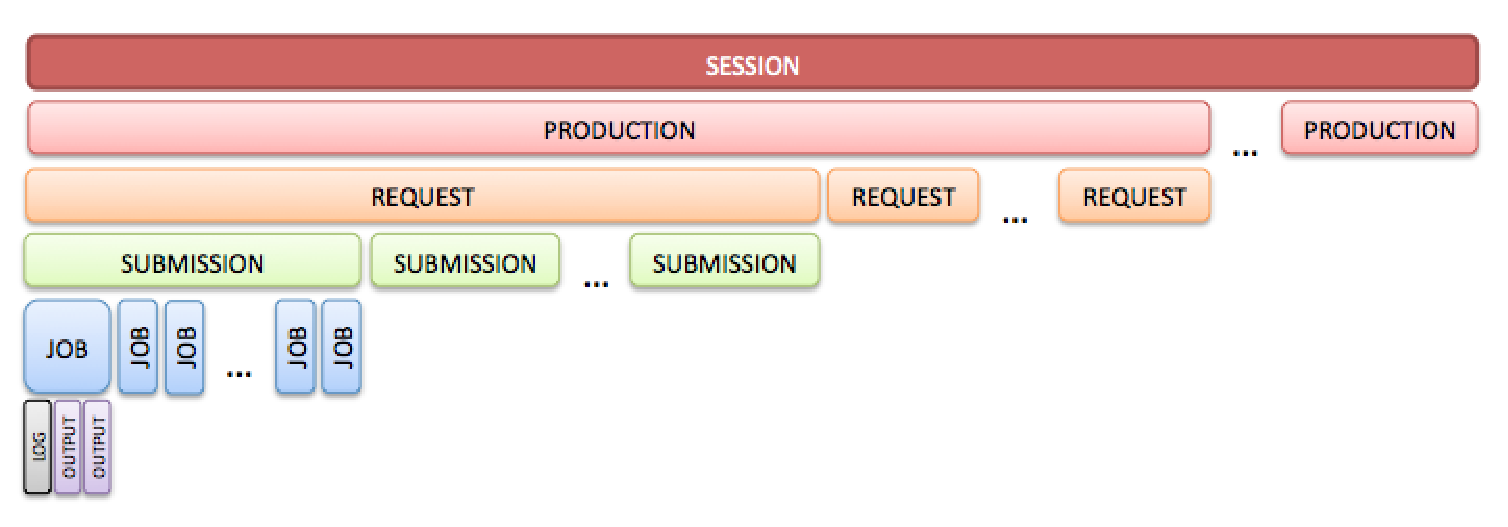
\includegraphics[width=3.5in]{BK_entities.eps}
\caption{Entities in BookKeeping database.}
\label{fig:BK_entities}
\end{figure}

Session defines a simulation (eg. FastSim and FullSim): parameters and software for simulation are defined by VO managers. Production is a Session subset that produce all the  needed to simulate a particular scenario (eg. background in detector).
Request is a Production subset. The required number of events to complete a Request is defined during its creation. Request completion is monitored via SBK, allowing job re-submission in order to complete it.\\
SBK design uses the relational model, and the current implementation relies on PostgreSQL (version 9.1) RDBMS which is SQL compliant and, exploiting its hstore datatype, allows to solve some major architectural issues concerning the dataset management of physical parameters. Hstore fields play a major role in the database architecture because storing sets of key/value pairs within a single PostgreSQL value is useful in various scenarios, such as rows with many attributes that are rarely examined, or semistructured data. Beside hstore, some other powerful PostgreSQL features have been exploited: its procedural language (PL/pgSQL) and schemas for a better management of user privileges. An extensive use of views and trigger procedures has been done too.

\subsection{Normalization studies}
During the development phase, the SBK database has been continuously analized in order to guarantee its normal form (NF) 1, 2 and 3 compliance. Four hierarchical levels (production, request, submission and ob+log+output+stat) have been identified for fastsim/fullsim to semplify table definitions and relations. In the production version the SBK database is NF1, NF2 and NF3 compliant with exception of hstore fields. A hstore is a string containing key->value couples and for this reason, if splitted into each couple key->value, it's not NF1 compliant. Since hstore fields permit to reduce database complexity and are rarely accessed (~100 updates every 6 months), a trade-off has been accepted keeping hstore columns not normalized.

\subsection{Stress tests}
Extensive stress tests to check PostgreSQL and HTTP REST interface system robustness have been carried out by means of the Tsung tool (http://tsung.erlang-projects.org/). Tsung allows to create virtual machines for testing scalability and performance of IP based client/server applications in order to do load and stress testing of servers. It can be distributed on several client machines and is capable to simulate hundreds of thousands of virtual users concurrently. For the test phase the REST interface has been configured to establish permanent DB connections to save connection slots. During the stress tests up to 100 users*s$^{-1}$ have been created. Each user has carried out a connection and 8 insert/update operations on a mock-up database which reproduced the real behavior of a production job. Stress test results were good, being the system capable to sustain 10000 DB transactions (1 transaction = 1 connection+8 insert/update) in ~100s (~900 operations*sec$^{-1}$).

\section{Bookkeeping DB integration}
\label{sec:db}

SBK integration in DIRAC is based on SQLAlchemy. SQLAlchemy uses Object Relational Mapper paradigm: database entities are mapped as python objects. SQLAlchemy adoption simplify code writing, reading and documenting, provides an abstraction layer capable to manage in a transparent way a wide variety of database backends, giving freedom to change it without needs to re-write code.
A new DIRAC service, named SBKService, integrates SQLAlchemy functionalities. SBKService interacts with other DIRAC components like any other service. SBKService maps SBK structure and expose methods to perform needed database operations.

\begin{figure}[!h]
\centering
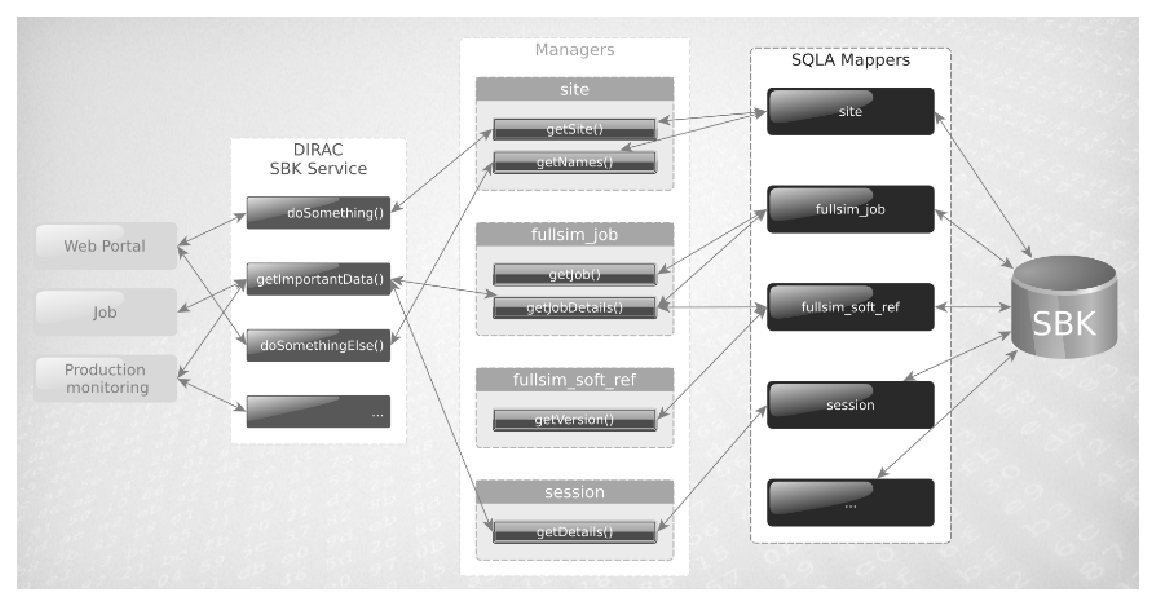
\includegraphics[width=3.5in]{SBKService.eps}
\caption{SBKService schema.}
\label{fig:SBKService}
\end{figure}

\section{Job wrapper component}
\label{sec:severus}

Job wrapper named Severus takes care of main operations of a simulation job: copy software and input files to WN, copy output files in SE and register them in LFC, copy log in SE and bookkeping DB, update job status in bookkeeping DB.

Access type (lcg or direct) from the worker node to the site SE is automatically recognized and implemented using lcg utils.
A module for each session takes care of properly setting environment variables according to simulation (aka session).
A configuration file customizes its behavior at execution time.
Configuration file has several sections:
\begin{itemize}
\item OPTIONS: general parameters
\item SOFTWARE: info about the executable
\item REST: info about the REST interface to be used for communications with DB
\item SITE: info about the submission site where the job will be running. A module for each site is loaded
\item TARGETSITE:  info about site where replicas of output files must be written
\item INPUT: info about the job input files
\item OUTPUT: info for stage-out phase
\item EXPORT VARS: list of environment vars to be exported on the WN
\item SESSION\_NAME: key-value pairs for simulation parameters, for the specified session
\end{itemize}

\begin{figure}[!h]
\centering
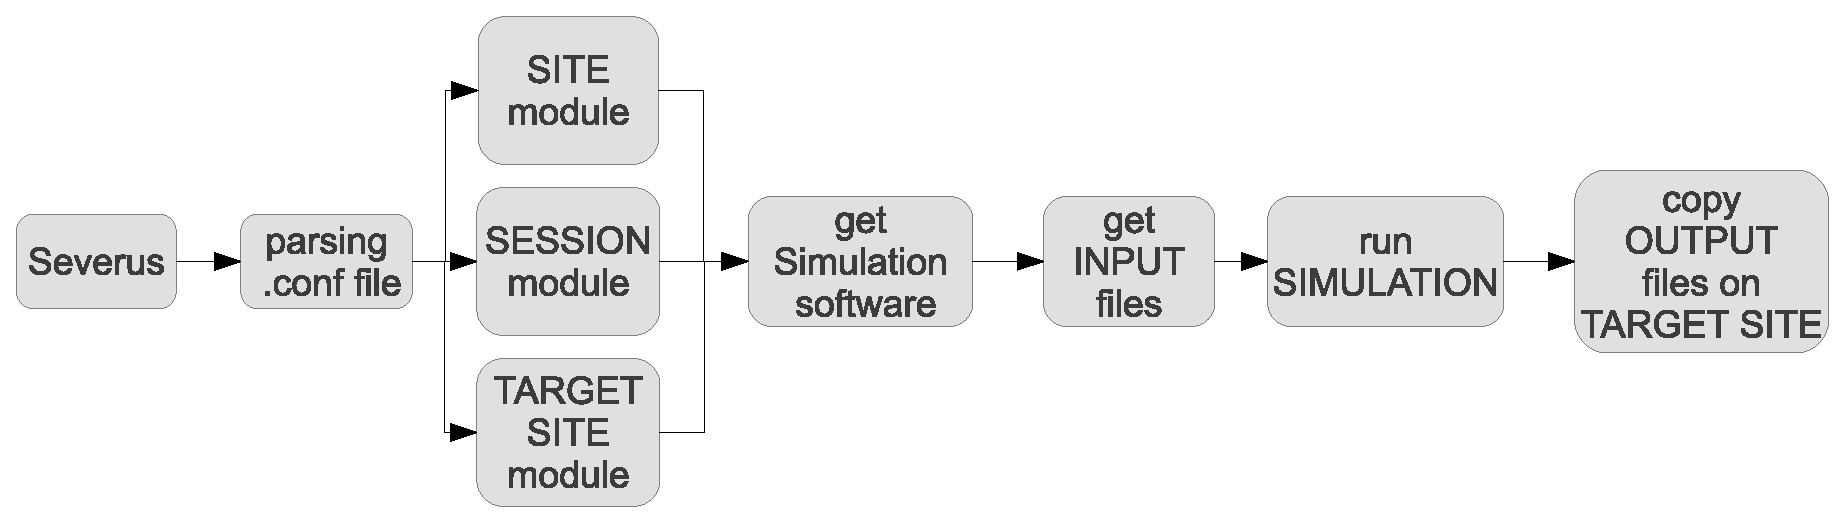
\includegraphics[width=3.5in]{severus_workflow.eps}
\caption{Severus workflow.}
\label{fig:severus_workflow}
\end{figure}

\section{Simulation production use case: the Super$B$ experience}
Simulation Production is designed to manage huge MonteCarlo productions.
A webportal, named WebUI\cite{ref:webui}, is available to manage the entire stack of operations related to this use case: user management, definition of new "Sessions", "Productions" and "Request", job submission and monitoring, sites management for productions. 
Production manager users can add and delete sites, add and delete CEs and SEs, set a site as enabled/disabled and supported/unsopported for a given session, manage "Sessions", "Productions" and "Request".
Shifter users can submit and monitor jobs for a given Request. Job submission in WebUI is performed via Ganga%\cite{ref:ganga}
, while submission configurations files are generated by WebUI itself taking data from SBK. Ganga submit jobs to grid via WMS using standard gLite commands. Job execution on WNs is driven by Severus (see section \ref{sec:severus}), while job status updates in SBK is performed via REST interface. Stagein and Stageout as well as output files registration in LFC is performed even by Severus. %See figure \ref{fig:simulation_production_workflow} for Simulation Production workflow.\\
SuperBDIRAC goal was the porting of the WebUI functionalities in DIRAC to manage jobs and their submission directly from DIRAC and exploit all the functionalities available in DIRAC: ie. Grid computing resources can be used via WMS or direct submission to CREAM CEs, computer clusters can be accessed via ssh connections, Cloud resources are available via VMDIRAC module, even desktop computers can be used via Boinc. User authentication via X509 certificates and authorization VOMS-role based are builtin in DIRAC.
SuperBDIRAC enhance DIRAC integrating the generic bookkeeping database SBK via SQLAlchemy.
DIRAC webportal is extended in order to provide an interface for Production manager actions as well as shifter tasks.

\begin{figure}[!h]
\centering
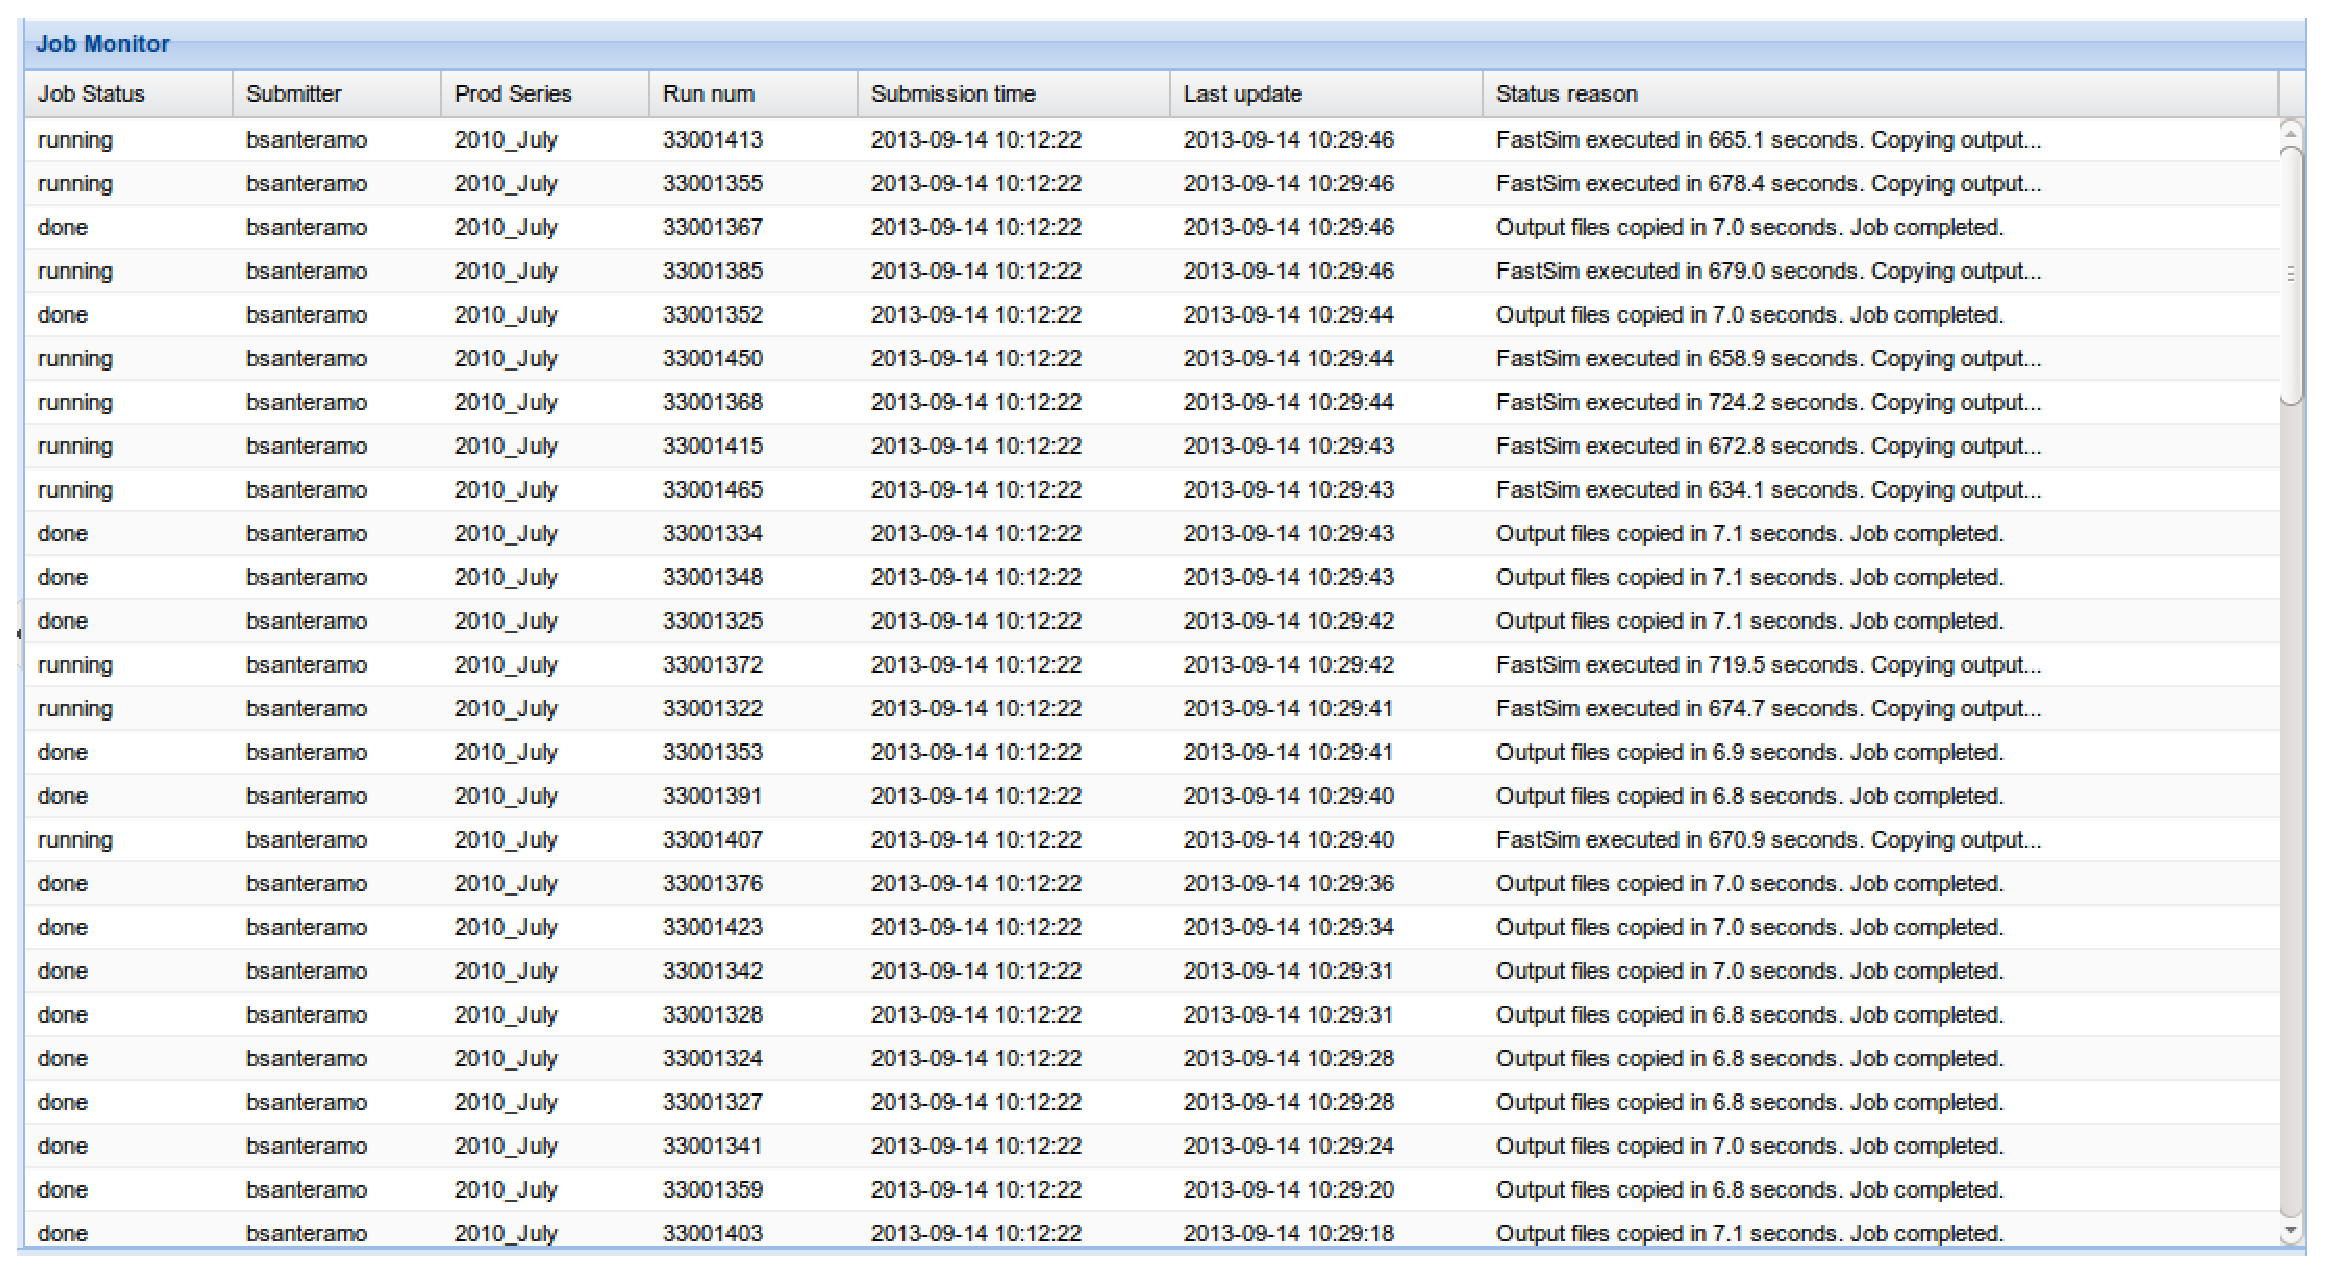
\includegraphics[width=3.5in]{SuperBDIRAC_monitoring.eps}
\caption{Monitoring job data from SBK in DIRAC.}
\label{fig:superbdirac_monitoring}
\end{figure}

\section{Functionality Test}
\label{sec:test}

A functionality test was performed to demonstrate the capability of SuperBDIRAC to integrate the monitoring of a bookkeeping database in DIRAC webportal.\\
Functionality Test objective is to demonstrate that SuperBDIRAC is capable of substituting WebUI as monitoring tool for job submission and showing data from a bookkeeping database. Test "Q-factor" is the exact correspondence of information as stored in SBK and displayed in SuperBDIRAC, like in WebUI monitoring page. Correct execution of simulation jobs is not important as long as the bookkeping information is properly managed.\\
At present time, not all WebUI functionalities are implemented in SuperBDIRAC, in particular "Submission" job for a given "Request".
The following procedure was used to perform this test. FastSim job submission is created via WebUI interface. Once submission is created, a set of scripts and configuration files are created. In particular the php submission script, generated by WebUI, is made of an array with all relevant parameters and UI commands needed to submit jobs in grid via standard glite commands.
Since WebUI is still linked with SBK, its portal could be used as well as monitoring portal, useful for a check-cross between info displayed in SBK, WebUI and SuperBDIRAC.\\

\begin{figure}[!h]
\centering
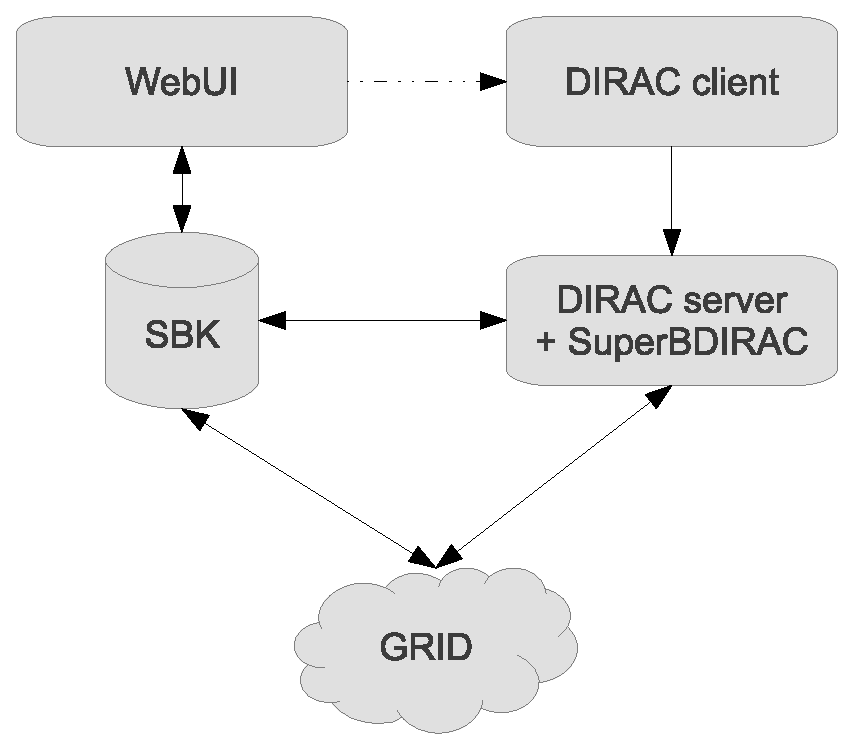
\includegraphics[width=3.5in]{testbed.eps}
\caption{Testbed schema.}
\label{fig:BK_entities}
\end{figure}

The php submission script is parsed by a python script (mc\_production.py), in particular the params array, in order to retrieve all needed parameters to properly submit jobs via DIRAC: production series, session name, min and max runnumber, configuration files location, physical parameters, events to simulate. Once taken all these parameters, mc\_production.py uses DIRAC API to prepare and submit jobs via DIRAC client.

DIRAC server receive jobs from DIRAC client, than starts the normal workflow for job management in DIRAC: scheduling, pilot submission, payload retrieval and execution, stageout. Since DIRAC server is equipped with SuperBDIRAC, even bookkeeping monitoring is performed by this component.
Every job simulated 3000 events: this value is set to have an execution time quite longer than 10 minutes.
Physical parameters are the same of other official productions.
3 main bunch submission of 400 jobs were performed at INFN-T1 to obtain a total of 1200 simulation jobs.
Status in SBK were "prepared", "running" and "done".
In addition, 2 bunch submission of 10 jobs were performed, again at INFN-T1, to force some failure messages in SBK and catch it even in SuperBDIRAC monitoring. First failure sample was obtained setting a not-existing site as destination for stageout: error was detected during preliminary check, so status in SBK were "prepared" and "failed". In second failure sample, jobs were submitted using a proxy without Role=ProductionManager, so error occurred in stageout phase: status in SBK were "prepared", "running" and "failed". In summary, 1220 jobs were submitted for test.\\

\begin{table}[h]\footnotesize
\begin{center}
    \begin{tabular}{|p{0.8cm}|p{0.4cm}|p{0.3cm}|p{0.3cm}|p{0.3cm}|p{0.3cm}|p{0.3cm}|p{0.3cm}|p{0.3cm}|p{0.3cm}|p{0.8cm}|}
    \hline
    & & \multicolumn{2}{ |c| }{prepared} & \multicolumn{2}{ |c| }{running} & \multicolumn{2}{ |c| }{done} & \multicolumn{2}{ |c| }{failed} & \\
    Test & Jobs & A & B & A & B & A & B & A & B & success rate\\
    \hline
    good-1 & 400 & 400 & 400 & 400 & 400 & 400 & 400 & 0 & 0 & 100\%\\
    good-2 & 400 & 400 & 400 & 400 & 400 & 400 & 400 & 0 & 0 & 100\%\\
    good-3 & 400 & 400 & 400 & 400 & 400 & 400 & 400 & 0 & 0 & 100\%\\      
    fail-1 & 10 & 10 & 10 & 0 & 0 & 0 & 0 & 10 & 10 & 100\%\\
    fail-2 & 10 & 10 & 10 & 10 & 10 & 0 & 0 & 10 & 10 & 100\%\\
    \hline
    \end{tabular}
\end{center}
\caption{Test results - A) expected B) test result}
\label{tab:status_update}
\end{table}


BookKeeping database was properly updated for every job in every test. All status change were promptly displayed as well in SuperBDIRAC as in WebUI, without any appreciable delay between two portals. SQLAlchemy didn't introduced any appreciable delay or information loss, at least in this functionality test. 
Table \ref{tab:status_update} reports, for every test, how many status were saved in SBK and displayed in WebUI and SuperBDIRAC. Success rate was established as ratio between status saved in SBK and status displayed in SuperBDIRAC: its value was 100\% in all submissions.
SuperBDIRAC could be considered good enough to integrate in DIRAC the capability of monitoring jobs metadata from a bookkeeping database.

\section{Conclusions}
DIRAC is a mature and stable framework to manage all grid-related tasks, easily adoptable by small as well large VOs.
The Information System is designed to be adapted for a generic huge simulation production.
The Job Wrapper acts as a bridge between simulation jobs and Information System.
We propose SuperBDIRAC as a DIRAC extension capable to satisfy the needs of small and mid size VOs in terms of distributed
resource exploitation.

%\appendices
%\section{}
%Appendices, if needed, appear before the acknowledgment.

% use section* for acknowledgement
%\section*{Acknowledgment}
%The preferred spelling of the word ``acknowledgment'' in American English is without an ``e'' after the ``g.'' Use the singular heading even if you have many acknowledgments. Avoid the expression, ``One of us (S.B.A.) thanks ...'' Instead, write ``S.B.A. thanks ...'' Put sponsor acknowledgments in the unnumbered footnote on the first page.


% references section

% can use a bibliography generated by BibTeX as a .bbl file
% BibTeX documentation can be easily obtained at:
% http://www.ctan.org/tex-archive/biblio/bibtex/contrib/doc/
% The IEEEtran BibTeX style support page is at:
% http://www.michaelshell.org/tex/ieeetran/bibtex/
%\bibliographystyle{IEEEtran}
% argument is your BibTeX string definitions and bibliography database(s)
%\bibliography{IEEEabrv,../bib/paper}
%
% <OR> manually copy in the resultant .bbl file
% set second argument of \begin to the number of references
% (used to reserve space for the reference number labels box)
\begin{thebibliography}{1}

\bibitem{ref:dirac} 
\verb"http://diracgrid.org"

\bibitem{ref:postgres}
\verb"http://www.postgresql.org/"

\bibitem{ref:sqlalchemy}
\verb"http://www.sqlalchemy.org/"

\bibitem{ref:boinc}
\verb"http://boinc.berkeley.edu/"

\bibitem{ref:superb_tdr}
Super$B$ Technical Design Report, \verb"http://arxiv.org/abs/1306.5655"

\bibitem{ref:rest}
Fielding R T 2000 {\it Architectural Styles and The Design of Network-based
Software Architectures }, PhD Thesis, University of California Irvine

\bibitem{ref:webui}
A.Fella, E.Luppi, L.Tomassetti \emph{A General Purpose Suite for Job Management, Bookkeeping and Grid Submission}. International Journal of Grid Computing \& Applications (IJGCA) Vol.2, No.2, June 2011. DOI: 10.5121/ijgca.2011.2202.

\end{thebibliography}


% that's all folks
\end{document}